\section{Design}
\label{sec:design}

Every structural decision follows from one sentence: the system is local-first, cloud-optional, and holds no scope the user has not explicitly granted. If the hypothesis is to be tested honestly, the restriction has to be structural rather than behavioural, impossible by construction rather than discouraged by instruction. This section describes the components that carry that requirement. Figure~\ref{fig:lifecycle} shows the path every request takes.

\begin{figure*}[t]
  \centering
  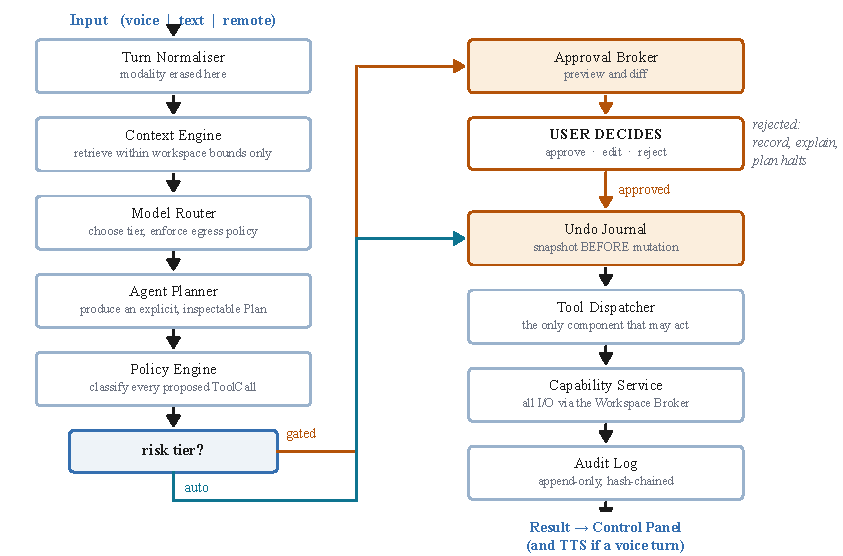
\includegraphics[width=0.78\textwidth]{figures/fig_lifecycle}
  \Description{Flow diagram: input is normalised, context is assembled within workspace bounds, a model tier is chosen, the planner produces a plan, the policy engine classifies each call; auto-approved calls go to the undo journal, dispatcher, capability service and audit log, while gated calls go through the approval broker and user decision first.}
  \caption{The request lifecycle. Modality is erased at the turn normaliser, so every stage below it is identical for voice and text. The gated branch returns beneath the undo journal, so an approved action is snapshotted before it is dispatched.}
  \label{fig:lifecycle}
\end{figure*}

\subsection{Request lifecycle and invariants}
A request, spoken or typed, local or from a paired device, is normalised into a modality-neutral turn, assembled into bounded context, planned as an ordered list of proposed tool calls, classified by the policy engine, held for approval where the verdict requires it, journalled for reversal, dispatched, and logged. Five invariants hold along this path, and each is directly testable: the policy engine is consulted before the dispatcher, never after; the undo journal snapshots before mutation, never after; an audit entry is written even when an action is rejected, so the log records what was proposed as well as what was performed; a tool call carrying no policy verdict is rejected by the dispatcher; and voice and text turns are indistinguishable from the planner onward. The planner, built on LangGraph~\cite{langgraph2024}, emits a plan and never executes one; the dispatcher executes and never decides. Separating the two is what makes the pause before any workspace-changing call structural rather than conventional. The planner's reflection loop is bounded by a cycle cap and a wall-clock budget, and a planner that cannot converge surfaces its partial plan and asks.

\subsection{Workspace broker}
The workspace broker is the only component that converts a logical reference into a filesystem path. It canonicalises the path, resolving symbolic links and relative segments, and only then asserts containment within a granted folder. The order matters: asserting first would allow a path that appears inside the grant to resolve outside it. A path outside every grant is not refused; it is unresolvable, and the attempt is logged. Capability services never touch the filesystem directly. The same boundary is enforced on the read side by the context engine, which tags every retrieved chunk with the workspace it came from and drops any chunk not matching the active grant before budgeting.

\subsection{Policy engine and risk tiers}
Every proposed tool call is classified into exactly one of four tiers (Figure~\ref{fig:tiers}). Reads (T0) run without a prompt. Reversible changes (T1), such as moving or creating a file, prompt according to user configuration. Outward actions (T2), such as sending mail or issuing a web query, always prompt regardless of configuration. Destructive actions (T3) are refused, and there is no approval dialogue for them because there is no code path to them. Rules are evaluated denials first, then gates, then permissions, so that no later rule can grant what an earlier rule refused. The option to approve and remember writes a rule scoped to this operation type, in this workspace, for this shape of action; it does not lower protection globally, which is the failure mode that turns permission systems into permanent consent. The graduation is a direct response to the formative finding that respondents split on asking first versus acting then undoing, and to the fatigue the security literature documents.

\begin{figure}[t]
  \centering
  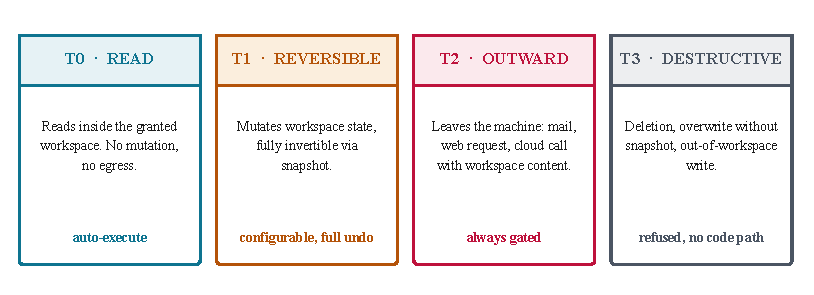
\includegraphics[width=\linewidth]{figures/fig_tiers}
  \Description{Four boxes labelled T0 read, T1 reversible, T2 outward and T3 destructive, with their handling: auto-execute, configurable with full undo, always gated, refused with no code path.}
  \caption{The four risk tiers. Only the reversible tier is user-configurable; outward actions are always gated, and destructive actions are refused structurally.}
  \label{fig:tiers}
\end{figure}

\subsection{Undo journal}
Before any reversible operation the journal records a forward and an inverse operation, choosing a snapshot strategy by cost: full content for small files, copy-on-write links for large ones, and inverse records alone for moves and renames. Undo operates at the granularity of a plan rather than of an operation, because a plan is the unit the user was asked to approve; reversing a folder tidy restores every move as one unit in reverse order. The formative study found that users forgive a mistake they can reverse, which makes a visible and reliable undo more valuable than an unattainable perfection.

\subsection{Disclosure}
A panel reports everything the system holds: granted workspaces, indexed files, embedded chunks, remembered facts, retained sessions, automation rules, policy exceptions, actions taken with their undo state, every record of data sent to a cloud provider, and the names of held credentials. It is a live query across every store, not a summary the system writes about itself, and every row is deletable with cascading effect. The design separates the file index, which is mechanical and rebuildable, from memory, which is interpretive and accumulates over sessions; the first requires only a grant, the second ongoing consent. The panel makes the trust claim falsifiable: a user can check it rather than believe it.

\subsection{Voice parity by construction}
Speech is not a capability service. It is normalised at the input layer into the same turn object as typed input and therefore inherits every approval gate automatically. If the voice path were a separate implementation, every gate would exist twice and the two copies would drift. Voice cannot approve, delete or send anything that typing cannot, and a voice session is explicitly armed and visibly indicated while active.

\subsection{Egress and prompt injection}
The model router owns tier selection and data egress. Local models are tried first through Ollama~\cite{ollama2024}, and cloud providers are reachable only when the active workspace permits them, in a configured order with one retry per tier. Retrieved documents, source code and web results can all be influenced by an adversary. The defence is not detection but the structural guarantee that retrieved content can never become an authorised instruction: provenance tagging of context, separation of the planner from untrusted data, the policy verdict on every call, approval of anything outward, and finally the workspace boundary, which bounds the worst case of any injection that defeats the preceding layers. That last layer is the strongest form of the hypothesis: confining the agent bounds the damage, not merely the expected behaviour.

\subsection{What the design does not solve}
Three limitations are inherited rather than solved. Approval fatigue is documented as an open problem in exactly the mechanism this design depends upon; the tiers reduce prompt frequency without eliminating the effect. The synthesis feature contains no faithfulness check, so unfaithful summaries remain possible over a narrower surface. The citation map carries each chunk back to its file, but nothing verifies that a citation supports the claim attached to it. All three are written into the evaluation as things to measure rather than assert away.
